%%%%%%%%%%%%%%%%%%%%%%%%%%%%%%%%%%%%%%%%%%%%%%%%%%%%%%%%%%%%%%%%%%%%%%%%%%%%%%%%
%%
%%   BornAgain Physics Manual
%%
%%   homepage:   http://www.bornagainproject.org
%%
%%   copyright:  Forschungszentrum Jülich GmbH 2015-2020
%%
%%   license:    Creative Commons CC-BY-SA
%%
%%   authors:    Scientific Computing Group at MLZ Garching
%%
%%%%%%%%%%%%%%%%%%%%%%%%%%%%%%%%%%%%%%%%%%%%%%%%%%%%%%%%%%%%%%%%%%%%%%%%%%%%%%%%

\def\Do{\overset{o}{D}}
\def\Go{\overset{o}{G}}
\def\TD{\TENS{D}}
\def\Td{\TENS{\delta}}
\def\TG{\TENS{G}}
\def\TU{\TENS{U}}
\def\TV{\TENS{V}}
\def\TL{\TENS{\Lambda}}
\def\TDo{\TENS{\overset{o}{D}}}
\def\TGo{\TENS{\overset{o}{G}}}
\def\vGo{\v{\overset{o}{G}}\vphantom{\v{G}}}
\def\Psio{\v{\overset{o}{\Psi}}\vphantom{\Psi}}
\def\ue{\v{\hat u}}

\def\pfo{\overset{o}{\psi}_\sf}
\def\pfoc{\overset{o}{\psi}\vphantom{\psi}^*_\sf}

\chapter{Scattering}\label{SSca}%
\chaptermark{Scattering}%
\index{Elastic scattering|seealso{Cross section}}%

This chapter provides a self-contained introduction
into the theory of neutron and X-ray scattering,
as needed for the analysis of grazing-incidence small-angle scattering (GISAS) experiments.
\index{Grazing-incidence small-angle scattering}%
\index{Scattering!grazing incidence|see{Grazing-incidence small-angle scattering}}%
\index{GISAS|see{Grazing-incidence small-angle scattering}}%
In \Cref{Swave},
a generic wave equation is derived.
In \Cref{SDWBA},
it is solved in first-order distorted-wave Born approximation (DWBA).
\index{DWBA|see {Distorted-wave Born approximation}}%
\index{Distorted-wave Born approximation}%
The chapter finishes with a qualitative discussion
of coherence lengths in \Cref{Scoherlen}.


%%%%%%%%%%%%%%%%%%%%%%%%%%%%%%%%%%%%%%%%%%%%%%%%%%%%%%%%%%%%%%%%%%%%%%%%%%%%%%%%
\section{Wave propagation}\label{Swave}
%%%%%%%%%%%%%%%%%%%%%%%%%%%%%%%%%%%%%%%%%%%%%%%%%%%%%%%%%%%%%%%%%%%%%%%%%%%%%%%%
\index{Wave propagation|(}%

In this section, we review the wave equations that describe the propagation
of neutrons (\cref{SnScalar,SnSpinor}) and X-rays (\cref{SXwave}) in matter,
and combine them into a unified wave equation (\cref{SuniWave})
that is the base for the all following analysis.
This provides justification and background
for Eqns.~1--3 in the BornAgain reference paper~\cite{PoVB20}.

%===============================================================================
\subsection{Neutrons}\label{SnScalar}
%===============================================================================
\index{Wave propagation!neutron|(}%
\index{Neutron!wave propagation|(}%

\def\Vmac{\tilde{V}}

\index{Schrodinger@Schrödinger equation!microscopic}%
The scalar wavefunction $\psi(\r,t)$
\nomenclature[2t020]{$t$}{Time}%
\nomenclature[2r040]{$\r$}{Position}%
\nomenclature[1ψ030 2r040 2t02]{$\psi(\r,t)$}{Microscopic neutron wavefunction}%
of a free neutron
in absence of a magnetic field
is governed by the Schrödinger equation
\begin{equation}\label{ESchrodi1}
  i\hbar\partial_t \psi(\r,t)
  = \left\{-\frac{\hbar^2}{2m}\Nabla^2+V(\r)\right\} \psi(\r,t).
\end{equation}
Since BornAgain only aims at modelling elastic scattering,
\index{Scattering!elastic}%
any time dependence of the potential is averaged out in the definition
\index{Potential!neutron}%
\index{Neutron!potential}%
$V(\r)\coloneqq \langle V(\r,t)\rangle$.
\nomenclature[2v130 2r040]{$V(\r)$}{Neutron potential}%
\index{Time dependence!neutron potential}%
Inelastic scattering,
\index{Inelastic scattering}%
\index{Scattering!inelastic}%
\index{Damping!inelastic scattering}%
\index{Loss terms|see {Damping}}%
in principle, can be accounted for by an extra contribution
damping.\footnote
{This is not explicitly supported in the software,
but users are free to increase the imaginary part of the refractive index
\index{Refractive index!losses from inelastic scattering}%
to emulate damping by inelastic losses.\label{Flosses}}
Therefore we only need to consider monochromatic waves
\index{Wave!monochromatic}%
\index{Monochromatic wave}%
with given frequency~$\omega$.
\nomenclature[1ω 020]{$\omega$}{Frequency of incident radiation}%
In consequence, the wavefunction
\begin{equation}\label{Estationarywave}
  \psi(\r,t) = \psi(\r)\e^{-i\omega t}
\end{equation}
\nomenclature[1ψ030 2r040 0]{$\psi(\r)$}{Stationary wavefunction}%
factorizes into a stationary wave and a time-dependent phase factor.
\index{Stationary wavefunction}%
\index{Phase factor}%
In the following, we will characterize the incoming radiation
not by its energy~$\hbar\omega$,
but by its \E{vacuum wavenumber}~$K$,
\index{Vacuum!neutron wavenumber}%
\index{Wavenumber!neutron}%
\nomenclature[2k120]{$K$}{Wavenumber in vacuum}%
given by the dispersion relation
\index{Dispersion relation!neutron}%
\index{Neutron!dispersion relation}%
\begin{equation}
  \hbar\omega = \frac{(\hbar K)^2}{2m}.
\end{equation}
The Schrödinger equation~\cref{ESchrodi1} then takes the simple form
\Emph{
\begin{equation}\label{ESchrodi2}
  \left\{\Nabla^2+K^2-4\pi v(\r)\right\} \psi(\r) = 0
\end{equation}
\vspace*{-5pt}}
with the rescaled form of Fermi's pseudopotential
\index{Fermi's pseudopotential}%
\index{Pseudopotential!Fermi's}%
\index{Potential!neutron}%
\index{Neutron!potential}%
\begin{equation}\label{Evrraw}
  v(\r)
  \coloneqq \frac{m}{2\pi\hbar^2} V(\r)
  = \sum_j\left\langle b_j \delta\left(\r-\r_j(t)\right)\right\rangle.
\end{equation}
The sum runs over all nuclei exposed to~$\psi$.
The \E{bound scattering length}~$b_j$
\index{Scattering length}%
\index{Bound scattering length|see{Scattering length}}%
\nomenclature[2b0]{$b$}{Bound scattering length}%
is isotope specific;
\index{Isotope}%
values are tabulated \cite{Sea92}.

In \E{small-angle scattering},
\index{Scattering!small-angle}%
\index{Small-angle scattering}%
\index{SAS|see{Small-angle scattering}}%
as elsewhere in \E{neutron optics} \cite{Sea89},
\index{Neutron!optics}%
\index{Optics!neutron}%
the potential can be coarse-grained by spatially averaging over at least a few atomic diameters,
\begin{equation}\label{Evrcoarse}
  v(\r)
  = \sum_s b_s \rho_s(\r),
\end{equation}
\nomenclature[2v030 2r040]{$v(\r)$}{Rescaled neutron potential, scattering length density (SLD)}%
where the sum now runs over chemical elements,
$b_s\coloneqq\langle b_j\rangle_{j\in s}$ is the bound \E{coherent} scattering length,
\index{Coherent scattering length}%
\index{Scattering length!coherent}%
and $\rho_s$ is a number density.
\index{Number density}%
\index{Density}%
\nomenclature[1ρ032 2s010]{$\rho_s$}{Number density of chemical element~$s$}%
In passing from \cref{Evrraw} to \cref{Evrcoarse},
we neglected \E{Bragg scattering}
\index{Scattering!Bragg}%
\index{Bragg scattering}%
from atomic-scale correlation,
\index{Atomic scale}%
\index{Correlation!atomic scale}%
and \E{incoherent scattering} from spin or isotope related fluctuations of $b_j$.
\index{Scattering!incoherent}%
\index{Incoherent scattering}%
\index{Isotope}%
\index{Spin!neutron}%
\index{Neutron!spin}%
In small-angle experiments,
 these types of scattering only matter as loss channels.\footnote
{Same remark as in \Cref{Flosses}: To model these losses, use the
\index{Refractive index!losses from Bragg scattering}%
\index{Refractive index!losses from incoherent scattering}%
imaginary part of the refractive index.}
Furthermore, incoherent scattering, as inelastic scattering,
 contributes to the diffuse background in the detector.
\index{Scattering!diffuse}%
\index{Scattering!inelastic}%
\index{Inelastic scattering}%
\index{Background!diffuse}%
\index{Detector!background}%
In conclusion, the coarse-grained neutron optical potential~\cref{Evrcoarse}
\index{Potential!optical}%
\index{Neutron!optical potential}%
\index{Neutron!potential}%
is just a \E{scattering length density} (SLD)
\index{Scattering length density}%
\index{SLD|see{Scattering length density}}%
\cite[eq.\ 2.8.37]{Sea89}.

In general, the incident neutron beam in a scattering experiment
is not a \E{pure} quantum state,
\index{Pure quantum state}%
\index{Quantum state!pure vs mixed}%
but a statistical mixture of such states,
\index{Mixed quantum state}%
and must therefore be described by a density matrix,
\index{Density matrix}%
\nomenclature[1ρ020]{$\hat\rho$}{Density matrix operator}%
\begin{equation}\label{EdefRho}
  \hat\rho \coloneqq \sum_j p_j \ket{\psi_j}\bra{\psi_j},
\end{equation}
where $p_j$ is the probability of pure state~$\psi_j$.
\nomenclature[2p022 2j000]{$p_j$}{Probability of state~$j$}%
Let us define the wave vector operator $\v{\hat k}$
\nomenclature[2k040]{$\k$}{Wave vector}%
and the flux operator
\begin{equation}\label{EdefJop}
  \v{\hat J} \coloneqq  \ket{\r}\bra{\r}\v{\hat k} + \v{\hat k}^\dagger\ket{\r}\bra{\r}.
\end{equation}
The current density, or \E{flux},
\index{Flux!neutron}%
\index{Current density|see{Flux}}%
is then given by
\begin{equation}\label{EdefJ}
  \v{J}(\r)
  \coloneqq \Tr\{\hat\rho \hat{\v{J}}\}
  \propto \sum_j p_j\left\{ \psi_j(\r)^*\frac{\Nabla}{2i}\psi_j(\r)
                        - \psi_j(\r)\frac{\Nabla}{2i}\psi_j(\r)^*\right\}.
\end{equation}
\nomenclature[2j150 2r040]{$\v{J}(\r)$}{Flux}%
This is in arbitrary units,
\index{Unit!neutron wavefunction}%
since we do not impose a specific normalization
\index{Normalization!neutron wavefunction}%
on the unbound wavefunction~$\psi$.
To compute scattering cross sections,
\index{Cross section}%
\index{Scattering!cross section}%
we will only need the \E{ratio} of scattered to incident flux.
Mostly we will assume pure states to be \E{plane waves}
\index{Plane wave}%
\index{Wave!plane}%
\begin{equation}\label{EplaneWave}
  \psi_\k(\r)\coloneqq\e^{i\k\r}.
\end{equation}
In vacuum, the wavevector~$\k$ purely real.
\index{Damping}%
We replace the sum in~\cref{EdefRho} by an integral,
and find that the flux is simply
\begin{equation}
  \v{J}(\r) = \int\!\d^3k\; p_\k\, |\psi_\k(\r)|^2 \k.
\end{equation}

%===============================================================================
\subsection{Neutrons in a magnetic field}\label{SnSpinor}
%===============================================================================

\index{Neutron!spin|(}%
\index{Spin|(}%
\index{Magnetic field!neutron propagation|(}%

\index{Field!magnetic|see{Magnetic field}}%
\index{H Field@$H$ Field|see{Magnetizing field}}%
\index{B Field@$B$ Field|see{Magnetic field}}%

In presence of a magnetic field,
the propagation of free neutrons becomes spin dependent.
Therefore the scalar wavefunction of \cref{SnScalar}
must be replaced by spinor $\v\Psi$.
\index{Spinor}%
The magnetic moment~$\mu$ of the neutron
\nomenclature[1μ024 2n000]{$\mu_\text{n}$}{Magnetic moment of the neutron}
\index{Neutron!magnetic moment}%
\index{Magnetic moment!neutron}%
couples to the magnetic induction~$\v{B}$ \cite{Mez86,MaOB06}.
\nomenclature[2h150 2r040 2t020]{$\v{B}(\r,t)$}{Magnetic induction}%
\index{Magnetizing field!coupling to neutron moment}%
With the coupling term, the Schrödinger equation~\cref{ESchrodi1}
\index{Schrodinger@Schrödinger equation!macroscopic}%
becomes
\begin{equation}\label{EHSchrodi}
  \left\{-\frac{\hbar^2}{2m}\Nabla^2+V(\r)
         +\mu\v{B}(\r)\bm{\hat\sigma}-\hbar\omega\right\}
      \v\Psi(\r) = 0,
\end{equation}
\nomenclature[1ψ150 2r040]{$\v\Psi(\r)$}{Stationary coherent spinor wavefunction}%
where $\mu_0$ is the vacuum permeability,
\nomenclature[1μ024 00]{$\mu_0$}{Vacuum permeability, $4\pi\cdot10^{-7}$ Vs/Am}%
\index{Permeability}%
\index{Magnetic permeability}%
and ${\bm{\hat\sigma}}$ is the Pauli vector, composed of the three Pauli matrices.
\nomenclature[1σ04]{$\bm\sigma$}{Pauli
    vector, composed of the three Pauli matrices: $\bm\sigma=(\sigma_x,\sigma_y,\sigma_z)$}%
\index{Pauli vector}%
\index{Pauli matrix}%
We introduce the reduced field
\begin{equation}
  \v{b} \coloneqq \frac{m\mu_0\mu_\text{n}}{2\pi\hbar^2}\v{B},
\end{equation}
\nomenclature[2h050 2r040]{$\v{b}(\r)$}{Rescaled
   field $\v{b}=(m\mu/2\pi\hbar^2)\v{B}$}%
\index{Magnetizing field!reduced}%
to rewrite the Schrödinger equation in analogy to~\cref{ESchrodi2} as
\index{Schrodinger@Schrödinger equation!macroscopic}%
\Emph{
\begin{equation}\label{ESchrodi2H}
  \left\{\Nabla^2+K^2-4\pi v(\r)-4\pi\v{b}(\r)\bm{\hat\sigma}\right\} \v\Psi(\r) = 0.
\end{equation}
\vspace*{-5pt}}
The density matrix~\cref{EdefRho} becomes
\begin{equation}\label{EdefRhoSpinor}
  \hat\rho \coloneqq \sum_i p_i \ket{\v\Psi_i}\bra{\v\Psi_i}.
\end{equation}
The total flux is still given by \cref{EdefJ,EdefJop}.
Beam polarization
\index{Polarization}%
is described by an appropriate density matrix.
\index{Neutron!spin|)}%
\index{Spin|)}%
\index{Magnetic field!neutron propagation|)}%

\index{Wave propagation!neutron|)}%
\index{Neutron!wave propagation|)}%

%===============================================================================
\subsection{X-rays}\label{SXwave}
%===============================================================================

\index{Wave propagation!X-ray|(}%
\index{X-ray!wave propagation|(}%

The propagation of X-rays is governed by Maxwell's equations,
\index{Maxwell's equations}%
\begin{equation}\label{EMaxwell}
  \begin{array}{@{}l@{\quad}l@{\quad}l}
    \Nabla\times\v{E}=-\partial_t \v{B},
   &\Nabla\v{B}=0,
   &\v{B}=\v{\mu}(\r)\mu_0\v{H},
   \\[2ex]
    \Nabla\times\v{H}=+\partial_t \v{D},
   &\Nabla\v{D}=0,
   &\v{D}=\v{\eps}(\r)\eps_0\v{E}.
  \end{array}
\end{equation}
\nomenclature[2e150 2r040 2t020]{$\v{E}(\r,t)$}{Electric field}%
\index{Electric field}
\nomenclature[2d150 2r040 2t020]{$\v{D}(\r,t)$}{Displacement field}%
\nomenclature[2b150 2r040 2t020]{$\v{B}(\r,t)$}{Magnetic field}%
\index{Magnetic field}
\index{Magnetizing field}
\nomenclature[1ε070 2r040]{$\v\eps(\r)$}{Relative dielectric permittivity tensor}%
\nomenclature[1μ070 2r040]{$\v\mu(\r)$}{Relative magnetic permeability tensor}%
\nomenclature[1ε024 00]{$\eps_0$}{Vacuum permittivity, 8.854\ldots As/Vm}%
Since BornAgain only addresses elastic scattering,
\index{Elastic scattering}%
\index{Scattering!elastic}%
we assume the permeability and permittivity tensors $\v\mu$ and~$\v\eps$
to be time-independent.
\index{Time dependence!dielectric permittivity}%
Therefore, as in~\cref{SnScalar}, we only need to consider monochromatic waves
\index{Wave!monochromatic}%
\index{Monochromatic wave}%
with given frequency~$\omega$,
and each of the fields $\v{E}$, $\v{D}$, $\v{H}$, $\v{B}$
factorizes into a stationary field and a time-dependent phase factor.\footnote
{This phase factor can be defined with a plus or a minus sign in the exponent.
Most texts on X-ray crystallography,
including influential texts on GISAXS \cite{ReLL09},
prefer the \E{crystallographic convention} with a plus sign.
\index{Wave propagation|seealso {Sign convention}}%
\index{Convention!sign convention}%
\index{Sign convention!wave propagation|(}%
\index{Crystallographic sign convention}%
In BornAgain, we prefer the opposite \E{quantum-mechanical convention}
\index{Quantum-mechanical convention}%
for consistency with the neutron case \cref{Estationarywave},
where the minus sign is an inevitable consequence
of the standard form of the Schrödinger equation.%
\index{Sign convention!wave propagation|)}%
}
\index{Phase factor}%
We will formulate the following in terms of the electric field
\index{Electric field}%
\begin{equation}\label{EstationaryX}
  \v{E}(\r,t) = \v{E}(\r)\e^{-i\omega t}.
\end{equation}
The other three fields can be obtained from~$\v{E}$
by straightforward application of~\cref{EMaxwell}.

Since magnetic refraction or scattering is beyong the scope of BornAgain,
the relative magnetic permeability tensor is always $\v{\mu}(\r)=1$.
\index{Permeability}%
\index{Magnetic permeability}%
As customary in SAXS and GISAXS,
\index{Grazing-incidence small-angle scattering!dielectric model}%
\index{Small-angle scattering!dielectric model}%
we assume
that the dielectric properties of the material are those of a polarizable electron cloud.\footnote
{This is occasionally called the \E{Laue model}
\index{Laue model}%
 \cite{Lau31}.}
Thereby the relative dielectric permittivity tensor~$\v{\eps}$
\index{Dielectric permittivity}%
\index{Permittivity}%
becomes a scalar,
\begin{equation}
  \eps(\r)=1-\frac{4\pi r_e}{K^2}\rho(\r),
\end{equation}
\nomenclature[1ε030 2r040]{$\eps(\r)$}{Relative dielectric permittivity function}%
\nomenclature[1ρ030 2r040]{$\rho(\r)$}{Electron number density}%
with the classical electron radius~$r_e=e^2/mc^2\simeq2.8\cdot10^{-15}$~m,
\index{Electron radius}%
\index{Classical electron radius}%
\nomenclature[2r024 2e000]{$r_e$}{Classical electron radius~$2.817\ldots^{-15}$~m}%
the electron number density~$\rho(\r)$,
\index{Electron density}%
\index{Density!electron}%
\index{Number density|see{Density}}%
and the vacuum wavenumber~$K$,
given by the dispersion relation
\begin{equation}
  K^2 = \mu_0\eps_0\omega^2.
\end{equation}
\index{Dispersion!X-ray}%

With these simplifying assumptions about $\v{\eps}$ and~$\v{\mu}$,
Maxwell's equations yield the wave equation
\begin{equation}\label{ENabCrossNabE}
  \Nabla\times\Nabla\times\v{E} = K^2\eps(\r)\v{E}.
\end{equation}
\index{Wave equation!X-ray}%
\index{X-ray!wave equation}%
Using a standard identity from vector analysis, it can be brought into the more tractable form
\Emph{
\begin{equation}\label{ENabNabE}
  \left\{\Nabla^2-\Nabla\cdot\Nabla+ K^2\eps(\r)\right\}\v{E}(\r)=0.
\end{equation}
\vspace*{-5pt}}

It is well known that the electromagnetic energy flux is given by the Poynting vector.
\index{Poynting vector}%
\index{X-ray!flux}%
\index{Flux!X-rays}%
However, its standard definition, $\v{S}\coloneqq\v{E}\times\v{H}$,
is not applicable here because it only holds for \E{real} fields.
With our complex notation, it must be replaced by
\begin{equation}
  \v{S}\coloneqq \Re\v E(\r,t)\times\Re\v H(\r,t).
\end{equation}
\nomenclature[2s150]{$\v S$}{Poyinting vector}%
For stationary oscillations~\cref{EstationaryX},
the time average is
\begin{equation}
  \braket{\v S} = \frac{1}{4}\braket{\v E(\r) \times \v H(\r)^* + \text{c.~c.}}.
\end{equation}
\nomenclature[2c000 2c000]{$\text{c.~c.}$}{Complex conjugate}%
We specialize to vacuum with $\TENS\mu(\r)=1$ and $\TENS\eps(\r)=1$,
and obtain
\begin{equation}
  \braket{\v S}
  = \frac{1}{4i\omega\mu_0}
    \left( \v E^*(\r)\times\left(\Nabla\times\v{E}(\r)\right) + \text{c.~c.} \right).
\end{equation}
For a plane wave $\v E(\r)=\v E_\k \e^{i\k\r}$, we find
\begin{equation}
  \braket{\v S}
  = \frac{1}{2\omega\mu_0} |\v E_\k|^2 \Re \k,
\end{equation}
which confirms the common knowledge that the radiation intensity
counted in a detector is proportional to the squared electric field amplitude.


\index{Wave propagation!X-ray|)}%
\index{X-ray!wave propagation|)}%

%===============================================================================
\subsection{Unified wave equation}\label{SuniWave}
%===============================================================================

As in Eqns.~1--3 of Ref.~\cite{PoVB20},
we combine all the above in a unified wave equation
\index{Wave equation!generic}%
\Emph{
\begin{equation}\label{EWAVE}
  \left( \TDo(\r) - 4\pi\TV(\r) \right) \v\Psi(\r) = 0
\end{equation}
\vspace*{-5pt}}
with the vacuum wave operator
\index{Vacuum!wave operator}%
\index{Wave!operator!vacuum}%
\begin{equation}\label{EDo}
  \TDo \coloneqq \left\{ \begin{array}{ll}
      \Nabla^2 + K^2                     &\text{~~~for neutrons,}\\
      \Nabla^2 - \Nabla\cdot\Nabla + K^2 &\text{~~~for X-rays}
  \end{array}\right.
\end{equation}
\nomenclature[2d138 0 2r040]{$\TDo(\r)$}{Differential operator in the vacuum wave equation}%
and the potential
\index{Potential!generic}%
\nomenclature[2v170 2r040]{$\TV(\r)$}{Generic potential}%
\begin{equation}\label{ETV}
  \TV(\r) \coloneqq \left\{ \begin{array}{ll}
      v(\r)                         &\text{~~~for neutrons (scalar),}\\
      v(\r)+\v{b}(\r)\bm\sigma       &\text{~~~for neutrons (spinorial),}\\
      K^2(\epsilon(\r)-1)/(4\pi) &\text{~~~for X-rays.}
  \end{array}\right.
\end{equation}
The generic wave amplitude $\v{\Psi}$
\nomenclature[1ψ150 2r040]{$\v\Psi(\r)$}{Generic wave amplitude,
  possibly vectorial or spinorial}%
shall represent
the scalar neutron wavefunction~$\psi$,
the spinor $\v{\Psi}$, or the electric field~$\v{E}$, as applicable.


%%%%%%%%%%%%%%%%%%%%%%%%%%%%%%%%%%%%%%%%%%%%%%%%%%%%%%%%%%%%%%%%%%%%%%%%%%%%%%%%
\section{Distorted-wave Born approximation}\label{SDWBA}
%%%%%%%%%%%%%%%%%%%%%%%%%%%%%%%%%%%%%%%%%%%%%%%%%%%%%%%%%%%%%%%%%%%%%%%%%%%%%%%%

To describe scattering from a condensed-matter sample,
\index{Scattering!target|see{Sample}}%
\index{Target|see{Sample}}%
\index{Sample}%
the wave equation is solved through a perturbation expansion.
The ordinary form of this expansion, the \E{Born approximation} (BA),
\index{BA|see{Born approximation}}%
\index{Born approximation}%
is derived in many textbooks.\footnote
{For a particularly detailed derivation
see Schober's lecture notes on neutron scattering~\cite{Sch14}.}
%E.~g.\ \cite{} for neutrons;
%\cite[Sect 9.7]{Jac75} for electromagnetic radiation}
For scattering under grazing-incidence,
\index{Grazing-incidence small-angle scattering}%
however, the more generic
\index{Distorted-wave Born approximation}%
\E{distorted-wave Born approximation} (DWBA)\footnote
{The DWBA was originally devised by Massey and Mott (ca 1933)
for collisions of charged particles.
Summaries can be found in some quantum mechanics textbooks (Messiah, Schiff)
and in monographs on scattering theory (e.~g.\ Newton).
The first explicit applications to grazing-incidence scattering
were published in 1982:
Vineyard \cite{Vin82} discussed X-ray scattering,
but failed to account for the distortion of the scattered wave;
Mazur and Mills \cite{MaMi82} deployed heavy formalism
to compute the inelastic neutron scattering cross section
of ferromagnetic surface spin waves from scratch.
A concise derivation of the DWBA cross section
was provided by Dietrich and Wagner (1984/85)
for X-rays \cite{DiWa84} and neutrons \cite{DiWa85}.
Unfortunately, their work was overlooked in much of the later literature,
which often fell back to less convincing derivations.}
is required.
In this section, we provide a self-contained derivation
based on the unified neutron and X-ray wave equation~\cref{EWAVE}.

%===============================================================================
\subsection{Distortion versus perturbation}\label{Sdecompose}
%===============================================================================

To get started,
we decompose the potential \cref{ETV}
into a more \E{regular} and a more \E{fluctuating} part:
\begin{equation}\label{Edecompose}
  \TV(\r) \eqqcolon \TL(\r) + \TU(\r).
\end{equation}
The \E{distortion field}~$\TL$
\index{Distortion field}%
\nomenclature[1λ170 2r040]{$\TL(\r)$}{Distortion field}%
comprises regular, well-known features of the sample.
The \E{perturbation potential}~$\TU$
\index{Perturbation potential}%
\index{Potential!perturbation}%
\nomenclature[2u170 2r040]{$\TU(\r)$}{Perturbation potential}%
stands for the more irregular, unknown features of the sample
one ultimately wants to study in a scattering experiment.
This is vague,
and in certain situations the decomposition~\cref{Edecompose} is indeed
to some extent arbitrary.
However, in most practical cases $\TL$ and $\TU$ are clearly determined by
the following basic idea of DWBA:

The wave equation~\cref{EWAVE} shall henceforth be written as
\Emph{
\begin{equation}\label{EDPsi}
  \TD(\r)\v\Psi(\r) = 4\pi\TENS{U}(\r)
\end{equation}
\vspace*{-5pt}}
with the \E{distorted wave operator}
\index{Distorted wave!operator}%
\index{Wave!operator!distorted}%
\nomenclature[2d138 2r040]{$\TD(\r)$}{Differential operator in the wave equation}%
\begin{equation}
  \TD(\r) \coloneqq \TDo - 4\pi\TL(\r).
\end{equation}
Only $\TENS{U}$ shall be treated as a \E{perturbation}.
The propagation of incident and scattered waves under the influence of~$\TL$,
in contrast,
shall be handled \E{exactly},
through analytical solution of the \E{unperturbed distorted wave equation}
\index{Unperturbed distorted wave equation}%
\index{Distorted wave!wave equation}%
\index{Wave equation!unperturbed distorted}%
\begin{equation}\label{EDPsi0}
  \TD(\r)\v\Psi(\r) = 0.
\end{equation}
The solutions are called \E{distorted}
\index{Distorted wave}%
\index{Wave!distorted}%
because they differ from the \E{plane} waves
\index{Plane!wave}%
\index{Wave!plane}%
obtained in the \E{vacuum} case $\TL=0$.
\index{Vacuum}%

Except for neutrons in a magnetic field
the distortion field is scalar so
that it can be expressed through the \E{refractive index}
\index{Refractive index}%
\index{Index of refraction|see {Refractive index}}%
\nomenclature[2n020]{$n$}{Refractive index}%
\begin{equation}\label{EnkK}
  n(\r)
  \coloneqq\sqrt{1-\frac{4\pi\Lambda(\r)}{K^2}}
  = \left\{\begin{array}{ll}
       \sqrt{1-4\pi\mv(\r)/K^2} &\text{ for neutrons,}\\
       \sqrt{\epsilon(\r)} &\text{ for X-rays.}
    \end{array}\right.
\end{equation}
If $\mv(\r)$ or $\epsilon(\r)$ has an imaginary part, describing absorption,
\index{Absorption}%
then $n(\r)$ is a complex number.
Conventionally, $n$ is parameterized by two real numbers:
\begin{equation}\label{Endb1}
  n \eqqcolon  1-\delta +i\beta.
\end{equation}
\nomenclature[1δ020]{$\delta$}{Small parameter in the refractive index
   $n=1-\delta +i\beta$}%
\nomenclature[1β020]{$\beta$}{Imaginary part of the refractive index}%
For thermal neutrons and X-rays,
$\delta$ and $\beta$ are almost always nonnegative,\footnote
{The plus sign in front of~$i\beta$ is a consequence of
the quantum-mechanical sign convention;
in the X-ray crystallography convention it would be a minus sign.
\index{Refractive index!sign convention}%
\index{Sign convention!refractive index}}
and much smaller than~1.
This explains why in most scattering geometries
\index{Scattering!geometry}%
the ordinary Born approximation
\index{Born approximation}%
with $\TL\equiv0$ is perfectly adequate.
In layered samples under grazing incidence,
\index{Grazing incidence}%
however, even small differences in~$n$ can cause substantial
\E{refraction} and \E{reflection}.
\index{Refraction}%
\index{Reflection}%
To model GISAS, therefore,
it is necessary to use DWBA,
\index{Distorted-wave Born approximation}%
and to let $\TL$ represent
the average vertical refractive index profile~$\overline{n}(z)$.
\index{Refractive index!profile}%

%===============================================================================
\subsection{The Rayleigh-Born expansion}\label{SBornExpans}
%===============================================================================

The solution of the wave equation~\cref{EDPsi}
starts with the determination of the \E{incident} wave~$\v\Psi_\si$.
\nomenclature[1ψ074 2i000 2r040]{$\v\Psi_\si(\r)$}{Incident wavefunction}%
\nomenclature[2i000]{i}{Subscript ``incident''}%
\index{Incident radiation!Born approximation}%
\index{Wave!incident}%
\index{Radiation|seealso{Wave}}%
\index{Incident wave!DWBA}%
\index{Incident wave!vs exciting wave}%
It is important to distinguish the \E{incident} from the \E{exciting} wave.
\index{Exciting wave}%
\index{Wave!exciting}%
They coincide in ordinary Born approximation, but not in DWBA.
\index{Born approximation}%,

The \E{exciting wave}
is prepared far
outside the sample by a radiation source and some optical devices.
\index{Radiation source}%
It is a superposition of plane waves,
as discussed later in the context of instrumental resolution effects
(\cref{SInstr}).
While discussing scattering theory,
it is usually represented by a single plane wave
$\v\Psi_\se(\r)=\e^{i\k_\se\r}$.
\nomenclature[1ψ134 2e000]{$\v\Psi_\se(\r)$}{Exciting wave}%
This function is defined for all~$\r$,
but is physical only along the primary beam, upstream of the sample.

The \E{incident wave}~$\v\Psi_\si$
\index{Incident wave!DWBA}%
\index{Incident wave!vs exciting wave}%
\index{Wave!incident}%
is an exact solution of~\cref{EDPsi0}
under the boundary condition that it must match~$\v\Psi_\se$
upstream of the sample.
Inside the sample it undergoes refraction and reflection
or other modifications under the influence of the distortion field~$\TL$.

A formal solution of the wave equation~\cref{EDPsi} is provided
by the \E{Lippmann-Schwinger equation}
\index{Lippmann-Schwinger equation}%
\begin{equation}\label{EPsiLS}
  \v\Psi(\r)
  = \v\Psi_\si(\r)
  + \int\!\d^3r'\, \TG(\r,\r') \TU(\r')\v\Psi(\r').
\end{equation}
It involves the Green function~$\TG$,
\index{Green function}%
\nomenclature[2g170 2r020 2r021]{$\TG(\r,\r')$}{Generic (possibly tensorial) Green function}%
which must fulfill
\begin{equation}\label{EGREEN}
  \TD(\r)\v\TG(\r,\r') = \ONE \delta(\r-\r') \eqqcolon \Td(\r-\r').
\end{equation}
To see that the Lippmann-Schwinger equation solves indeed the perturbed wave equation~\cref{EDPsi},
operate on both sides of~\cref{EPsiLS} with~$\TD(\r)$.
The Lippmann-Schwinger equation can be resolved into an infinite series
by iteratively substituting the full right-hand side of~\cref{EPsiLS}
for the occurence of~$\v\Psi$ in the integrand.
\index{Perturbation expansion}%
\index{Born!expansion (or series)}%
This is the \E{Born expansion} or \E{Born series}.\footnote
{Named after Max Born who introduced it in quantum mechanics.
It is actually due to Lord Rayleigh who devised it for sound,
and later also applied it to electromagnetic waves,
which resulted in his famous explanation of the blue sky.}
Successive terms in this series contain rising powers of $\TU$.
As long as $\TU$ is a small perturbation, the series converges quickly.
In \E{first-order Born approximation},
\index{Born approximation}%
only the linear order in $\TU$ is retained,
\begin{equation}\label{EBorn}
  \v\Psi(\r)
  = \v\Psi_\si(\r)
  + \int\!\d^3r'\, \TG(\r,\r') \TU(\r')\v\Psi_\si(\r').
\end{equation}
This is the base for material investigations with X-rays or neutrons,
where sample structures that modulate the perturbation potential $\TU$
are deduced from the scattered intensity ${|\v\Psi(\r)|}^2$.
Since detectors are always placed at positions $\r$
that are not illuminated by the incident beam,
we are only interested in the scattered wave
\index{Scattered radiation!Born approximation}%
\index{Wave!scattered}%
\Emph{
\begin{equation}\label{EBornS}
  \v\Psi_\text{s}(\r)
  \coloneqq
  \int\!\d^3r'\, \TG(\r,\r') \TU(\r') \v\Psi_\si(\r').
\end{equation}
\vspace*{-5pt}}
\nomenclature[1ψ034 2s000 0 2r040]{$\psi_\text{s}(\r)$}{Scattered wavefunction}%
\nomenclature[2s000 0]{s}{Subscript ``scattered''}%
For brevity and mathematical convenience,
the integral has no bounds
and therefore formally runs over the entire space.
However, $\TU(\r')$ is nonzero only if $\r'$ lies inside the finite sample volume.

%===============================================================================
\subsection{Far-field Green function}\label{SDWGreen}
%===============================================================================

In experiments, scattered radiation is measured
at a detector position~$\r$ so far outside the sample
that the distance from the sample to the detector
is must be much larger than the size of the sample.
This is just the condition for \E{Fraunhofer diffraction};
\index{Fraunhofer approximation}%
In scattering theory,
it is known as the \E{far-field approximation}.
\index{Far-field approximation}%
We choose the coordinate origin
\index{Coordinate system!origin}%
\index{Origin!coordinate system}%
inside the sample so that the far-field asymptote corresponds to the limit $r\to\infty$.
To determine the far-field asymptote $\v\Psi_\text{s}^\infty(\r)$
of the scattered wave~$\v\Psi_\text{s}$ from~\cref{EBornS},
\index{Scattered radiation!far field}
it is sufficient to solve~\cref{EGREEN} for the far-field Green function
\begin{equation}\label{EGinftydef}
  \TG^\infty(\r,\r')\coloneqq \lim_{r\to\infty} \TG(\r,\r').
\end{equation}
\nomenclature[2g174 2far]{$\TG^\infty(\r,\r')$}{Far-field
   approximation to the Green function $G(\r,\r')$}%

%--------------------------------------------------------------------------------
\begin{figure}[tb]
\begin{center}
\includegraphics[width=1\textwidth]{fig/drawing/Green1.ps}
\end{center}
\caption{(a)
The Green function $G(\rS,\rD)$
\index{Green function}%
is the probability that radiation emitted
by a source~S is reaches a detector~D.
If S is a locus of scattering in a multilayer sample,
then $G$ is a sum over different trajectories,
\index{Trajectory}
involving refraction and reflection
at layer interfaces.
(b) For the far-field
\index{Far-field approximation!Green function}%
Green function $G_\infty(\rS,\rD)$,
the detector is moved so far away from the sample
that all trajectories are practically parallel when they leave the sample.}
\label{Fgreen1}
\end{figure}
%--------------------------------------------------------------------------------

In deriving~$\TG^\infty$, it is preferable to work with well-defined
\E{polarization states}.
\index{Polarization!state}%
For either neutron spinors or electric fields,
the scattered field amplitude in vacuum
can be written as sum over two orthogonal states~$\alpha$
\nomenclature[1α010]{$\alpha$}{Polarization state index}%
with unit amplitudes~$\ue_\alpha$:
\nomenclature[2u041]{$\ue$}{Polarized field amplitude unit vector}%
\begin{equation}
   \v\Psi_\text{s}(\r)
   = \sum_\alpha\ue_\alpha\psi_\text{s}^\alpha(\r)
\end{equation}
with
\begin{equation}
  \psi_\text{s}^\alpha(\r)
  \coloneqq \ue_\alpha^* \v\Psi_\text{s}(\r).
\end{equation}
Similarly, we introduce the vectorial Green function with final polarization state~$\alpha$,
\begin{equation}
   \v{G}^\alpha(\r,\r')
   \coloneqq \ue_\alpha^* \TG(\r,\r').
\end{equation}
In the far-field limit, it is given by\footnote
{To our knowledge,
the simple expression \cref{EmyG} has never before been stated.
Informations about similar results anywhere in the literature would be highly welcome.}
\Emph{
\begin{equation}\label{EmyG}
  \v{G}^\infty_\alpha(\r,\r') = \phi(r) \v\Psi_\alpha^*(\r'),
\end{equation}
\vspace*{-5pt}}
where $\phi$ is an outgoing spherical wave with
\begin{equation}\label{Effphidef}
  \phi(r) \coloneqq \frac{\e^{iKr}}{4\pi r},
\end{equation}
and $\v\Psi_\alpha$ is a solution of the unperturbed distorted wave equation
\begin{equation}
  \TD(\r)\v\Psi_\alpha(\r) = 0
\end{equation}
with the boundary condition
\begin{equation}
  \v\Psi_\alpha(\r) = \ue_\alpha\e^{i\k_\sf\r}
\end{equation}
for $r\to\infty$ and
with an outgoing wavevector
\nomenclature[2f000]{f}{Subscript ``final''}%
$\k_\sf\coloneqq K \r / r$.

We now outline a proof for~\cref{EmyG}.
We take for granted that Green functions obye \E{source-detector reciprocity} \cite{Pot04},
\begin{equation}
  \TG(\r,\r') = \TG(\r',\r).
\end{equation}
We first consider wave propagation in vacuum,
denoted by an overset circle.
Exact Green functions
are known.
The far-field must be taken explicitly,
and in all cases
\begin{equation}
  \vGo_\alpha^\infty(\r,\r') = \phi(r)\Psio_\alpha^*(\r')
\end{equation}
is obtained.
Following Dietrich and Wagner \cite{DiWa84,DiWa85,DiWa16},
we write Lippmann-Schwinger equations for a distorted wave
\begin{equation}\label{ELS2Psi}
   \Psio_\alpha(\r)
   = \int\!\d^3r''\, \left( \delta(\r-\r'') + \vGo_\alpha(\r,\r'')4\pi\TL(\r'') \right)
                     \v\Psi_\alpha(\r''),
\end{equation}
and for the Green function
\begin{equation}\label{ELS2G}
   \vGo_\alpha(\r,\r')
   = \int\!\d^3r''\, \left( \delta(\r-\r'') + \vGo_\alpha(\r,\r'')4\pi\TL(\r'') \right)
                     \v{G}_\alpha(\r'',\r').
\end{equation}
Operate on both sides with~$\TDo(\r)$ to verify that
\begin{equation}
  \TDo(\r)\TGo(\r,\r') = \Td(\r-\r') \text{ and } \TDo(\r)\Psio(r)=0
\end{equation}
imply
\begin{equation}
  \TD(\r)\TG(\r,\r') = \Td(\r-\r') \text{ and } \TD(\r)\v\Psi(r)=0.
\end{equation}
To continue, use the reciprocity of the Green function,
and take the far-field limit to transform~\cref{ELS2G} into
\begin{equation}\label{ELS2G2}
   \phi(r')\Psio_\alpha^*(\r)
   = \int\!\d^3r''\, \left( \delta(\r-\r'') + \vGo_\alpha(\r,\r'')4\pi\TL(\r'') \right)
                     \v{G}_\alpha^\infty(\r',\r'').
\end{equation}
Take the complex conjugate of~\cref{ELS2Psi},
multiply with~$\phi(r')$, and compare with \cref{ELS2G2}
to read off
\begin{equation}
   \v{G}_\alpha^\infty(\r',\r'') = \phi(r')\v\Psi_\alpha(\r''),
\end{equation}
which is~\cref{EmyG}.

%===============================================================================
\iffalse
\subsection{Reciprocity of the Green function}\label{SReci}
%===============================================================================

\index{Reciprocity|(}%
\index{Green function!reciprocity|(}%

Our computation of~$G_\infty$ will be based on a source-detector \E{reciprocity theorem}
for the scalar Schrödinger equation.\footnote
{There exists a confusing multitude of reciprocity theorems \cite{Pot04}.
In the end, we found it simpler to provide a derivation taylored for our application case
than to refer to the literature.}
The theorem states:
Any Green function $G(\r,\r')$
that solves~\cref{EGREEN} and as function of~$\r$ represents an outgoing wave
%(in accord with the Sommerfeld radiation condition)
%\index{Sommerfeld radiation condition}%
is invariant under an exchange of source location~$\rS$ and detection point~$\rD$:
\nomenclature[2r041 2d100]{$\rD$}{Position of detector}%
\nomenclature[2r041 2s100]{$\rD$}{Position of source, locus of scattering}%
\begin{equation}\label{Erecip}
  G(\rS,\rD) = G(\rD,\rS).
\end{equation}
Readers not interested in mathematical details may skip the following \E{proof}:

We introduce the auxiliary vector field
\begin{equation}
  \v{X}(\r,\rS,\rD)\coloneqq G(\r,\rD)\Nabla G(\r,\rS) - G(\r,\rS)\Nabla G(\r,\rD).
\end{equation}
%\nomenclature[2x150 2r040]{$\v{X}(\r,\rS,\rD)$}{Auxiliary vector field}%
We inscribe the sample and the detector
into a sphere $\Sphere$ around the coordinate origin with radius~$R$,
%\nomenclature[2s180]{$\Sphere$}{Auxiliary spherical volume}%
%\nomenclature[2r120]{$R$}{Radius of $\Sphere$}%
and compute the volume integral
\begin{equation}\label{Eprerecipro}
    I(\rS,\rD) \coloneqq \displaystyle\int_\Sphere\!\d^3r\,\Nabla \v{X}(\r,\rS,\rD).
\end{equation}
After a few steps, not entirely trivial, but not too difficult either,
we obtain
\begin{equation}\label{EIBD}
  I(\rS,\rD) = G(\rS,\rD) - G(\rD,\rS).
\end{equation}
Alternatively, we can compute $I$ as a surface integral
\begin{equation}
  I(\rS,\rD)
  =\displaystyle\int_{\partial\Sphere}\d\v{\sigma}\,\v{X}(\r,\rS,\rD).
\end{equation}
On the surface $\partial\Sphere$,
$G$ is an outgoing solution of the Helmholtz equation.
As such, it has a well-known series expansion in spherical coordinates.
We send $R\to\infty$ so that we need only to retain the lowest order:
\begin{align}
   G(\r(R,\vartheta,\varphi),\rD)
   &\doteq\displaystyle \frac{\e^{iKR}}{4\pi R} a(\vartheta,\varphi),
   \\[3.8ex]
   G(\r(R,\vartheta,\varphi),\rS)
   &\doteq\displaystyle \frac{\e^{iKR}}{4\pi R} b(\vartheta,\varphi).
\end{align}
The factorization of $G$ and $B$ and their common $R$ dependence imply that
\begin{equation}
  I(\rS,\rD)
  =\displaystyle\int_{\partial\Sphere}\d\sigma\,
       (\text{$R$-dependent})(ab-ba)
  = 0.
\end{equation}
Comparison with \cref{EIBD} yields \cref{Erecip},
which completes the proof.

\index{Reciprocity|)}%
\index{Green function!reciprocity|)}%
\fi

%===============================================================================
\subsection{Differential cross section}\label{SdiffCross}
%===============================================================================

\index{Flux!incident and scattered}%
The ratio of the scattered flux hitting an infinitesimal detector area
$r^2\d\Omega$ to the incident flux is expressed as a
\E{differential cross section}
\index{Cross section}%
\index{Scattering!cross section}%
\index{Incident radiation!flux|(}%
\begin{equation}\label{Exsectiondef}
  \xElas
  \coloneqq  \frac{r^2 J(\r)}{J_\si}.
\end{equation}
\nomenclature[1ω120]{$\Omega$}{Solid angle}%
\nomenclature[1σ020]{$\sigma$}{Scattering or absorption cross section}%
% TODO RESTORE XREF
% The geometric factors that are needed to
% convert $\d\sigma/\d\Omega$ into detector counts will be discussed
% below in \cref{SdetImg}.
For a plane wave~\cref{EPsi0Plane}, the incident flux is
\index{Incident radiation!flux|)}%
\index{Flux!Born approximation}%
\begin{equation}\label{EJi}
  \v{J}_\si = \k_\si.
\end{equation}
With the far-field result~\cref{EsandwichC}
and the notation~\cref{Etrama},
the scattered flux at the detector is
\begin{equation}\label{EJr}
  \v{J}(\r)
  = \v{\hat r}\frac{K}{r^2}
    {\left|\braket{\psi_\si|\delta v|\psi_\sf}\right|}^2.
\end{equation}
\index{Scattered radiation!flux}%
Inserting these into definition~\cref{Exsectiondef},
we obtain the generic differential cross section
of elastic scattering in first order Born approximation,
\index{Born approximation!elastic scattering cross section}%
\index{Cross section!Born approximation}%
\index{Scattering!cross section}%
\Emph{
\begin{equation}\label{Exsection}
  \xElas
  =  {\left|\braket{\psi_\si|\delta v|\psi_\sf}\right|}^2.
\end{equation}\vspace*{-5pt}
}
As we shall see below,
it holds not only for plane waves governed
by the Helmholtz equation,
but also for distorted waves.
\index{Distorted-wave Born approximation!elastic cross section}%
In the plane-wave case \cref{Echiq} considered here,
the differential cross section is just the squared modulus
of the Fourier transform of the SLD,
\index{Scattering!length density!Fourier transform}%
\begin{equation}\label{Ecross1}
  \xElas
  = {\left| v(\q) \right|}^2.
\end{equation}

%%%%%%%%%%%%%%%%%%%%%%%%%%%%%%%%%%%%%%%%%%%%%%%%%%%%%%%%%%%%%%%%%%%%%%%%%%%%%%%%
\section{Coherent vs incoherent scattering}\label{Scoherlen}
%%%%%%%%%%%%%%%%%%%%%%%%%%%%%%%%%%%%%%%%%%%%%%%%%%%%%%%%%%%%%%%%%%%%%%%%%%%%%%%%

%===============================================================================
\subsection{Coherence length}
%===============================================================================

Per \cref{Exsection} and~\cref{Etrama},
\index{Coherence length|(}%
the matrix element $\braket{\psi_\si|\delta v|\psi_\sf}$
is given by a three-dimensional integral
\begin{equation}\label{Etrama3}
  \braket{\psi_\si|\delta v|\psi_\sf}
  \coloneqq  \int\!\d^3r\, \psi^{*}_\si(\r)\delta v(\r)\psi_\sf(\r).
\end{equation}
The integration domain is effectively limited to a finite $z$ interval,
where $\delta v(\r)$ is nonzero.
The horizontal integration domain, however, is infinite
within our formalism,
which is of course an idealization.
Obviously, physical integration limits are imposed by the finite
\index{Sample area}%
\E{illuminated sample area}.\footnote
{We assume a well aligned instrument,
for which the beam footprint and the backtracked detector footprint
\index{Illumination!beam footprint on sample}%
\index{Beam footprint}%
\index{Backtracking!beam footprint}%
agree within reasonable accuracy.}
Another limitation comes from the finite \E{coherence length}
of the instrumental setup,
which usually is much shorter than the sample width and length
%This is of importance in neutron scattering
%where typical sample dimensions of 1\ldots10~mm
%are much larger than the relevant coherence length,
%which is of the order 10\ldots100~$\upmu$m
\cite{HaPR10,MaMM14}.\footnote
{These two references also make clear that
  the theoretical description and the experimental determination of
  coherence lengths are difficult problems and subject of ongoing research.}

While each single neutron is described by a wavefunction
that allows for \E{coherent} superposition of
different contributions to the scattered wavefunction,
the final detector statistics
\index{Detector!statistics}%
is given by an \E{incoherent} sum
over the differential cross sections of individual neutrons.
The finite \E{resolution}
\index{Resolution|(}%
of an experimental setup is in part due to the fact that
different neutrons have different wavenumbers,
originate\footnote
{It is reasonable to take the last collision in the moderator
  as the \E{origin} of a neutron ray,
  since collisions between neutrons and hydrogen nuclei bound in
  disordered matter lead to almost perfect decoherence.}
at different points in the moderator,
and are detected at slightly different points within one detector pixel.
This can be modeled by computing expected scattering intensities as
averages over different neutrons with
$K$, $\v{\hat k}_\si$, and $\v{\hat k}_\sf$ drawn at random
from appropriate distributions.
% TODO RESTORE TEMPORARILY REMOVED XREF as described in \cref{Sresolution}.

However, this is not the full story.
In the above introduction to the Born approximation
we have made the standard assumption
that an incoming neutron can be described by a plane wave
$\psi_\si=\e^{i\k_\si\r}$.
The wavefunction $\psi_\sf$ traced back from the detector is also
approximated by a plane wave.
In the DWBA we allow these waves to be distorted within the sample,
but when impinging on the sample they still are plane.
A plane wave obviously is an idealized concept,
since it has infinite lateral extension.
The \E{transverse coherence length} indicates the scale
beyond which this approximation becomes invalid.
At larger scales, the wave fronts appear randomly distorted.
Physical causes of these distortions include
reflections in the neutron guide,
diffraction by guide windows and other slits,
and diffraction by imperfect monochromator crystals.
Of course the distorted wave still admits a Fourier decomposition
into plane waves with slightly different wavevectors.
In practice, it is impossible to distinguish this spread of wavevectors
from the incoherent spread described in the previous paragraph.
The instrumental resolution function therefore
accounts for both causes of wavevector distortion.
\index{Resolution|)}%

Usually, therefore, a GISANS image is an incoherent average
over coherent diffraction patterns collected from
many small subareas of the sample.
Only horizontal sample structures on scales smaller the coherence length
yield interference patterns.
Structure fluctuations on larger scales
produce said incoherent average of different GISANS images.

The crossover from coherent to incoherent scattering is of course
a gradual one.
The coherence length indicates where a certain, somewhat arbitrary degree
of decoherence is reached.
Under these reservations
one defines a \E{coherence spot}
in the cross section of an approximately plane wave
as an area where the coherence is above a certain threshold.
Unless the wave has been prepared in a highly anisotropic guide and slit system,
this spot is about circular.
Under grazing incidence conditions however,
the projection of this spot onto the sample surface
yields a very elongated ellipse.
Therefore, the coherence length is much larger in $x$ than
in $y$ or $z$ direction.\footnote
{This has nothing to do with the distinction of
  \E{transverse} and \E{longitudinal} coherence length.
  Longitudinal coherence has to do with wavelength stability
  and is of no importance for elastic scattering.
  We are talking here about \E{horizontal} and \E{vertical}
  projections of the \E{transverse} coherence length.}

%===============================================================================
\subsection{Implementation}
%===============================================================================


\Note{\indent Unless otherwise said, \BornAgain\ simulates
  \E{coherent} diffraction patterns obtained by
  the linear superposition of scattered waves.
  To simulate an \E{incoherent} mixture of diffraction patterns,
  the most generic solution is a script with an outer loop
  that averages over several coherent computations with
  appropriately distributed parameters.}

\Warn{\indent Currently, \BornAgain\ does not support interferences
  between particles in different layers.}
% TODO: more about implementation !

\index{Coherence length|)}%




%%%%%%%%%%%%%%%%%%%%%%%%%%%%%%%%%%%%%%%%%%%%%%%%%%%%%%%%%%%%%%%%%%%%%%%%%%%%%%%%
\section{OLD STUFF}
%%%%%%%%%%%%%%%%%%%%%%%%%%%%%%%%%%%%%%%%%%%%%%%%%%%%%%%%%%%%%%%%%%%%%%%%%%%%%%%%

NOMENCLATURE STUFF
\nomenclature[1ε031 2r040]{$\overline\eps(\r)$}{Part of the permittivity~$\eps(\r)$ that can be analytically handled}%
\nomenclature[1δ030
  1ε030 2r040]{$\delta\eps(\r)$}{Part of the permittivity~$\eps(\r)$ that causes scattering}%

The SLD fluctuations can typically written as a sum over different materials~$p$,
\begin{equation}
  \delta v(\r) = \sum_p (v_p-\mv(\r)) \chi_p(\r),
\end{equation}
where $v_p$ is the SLD of the bulk material~$p$,
and $\chi_p$ is dimensionless function that takes values between 0 and~1.
Internally, BornAgain computes $v_p$ from the material's refractive index,
\begin{equation}
  v_p = \frac{K^2}{4\pi}(1-n_p).
\end{equation}

Absolute values of~$U(\r)$ are always much smaller than~1.
This enables us to solve \cref{EDPsi} by a first-order perturbation theory,
\index{Perturbation expansion}%
the \E{distorted-wave Born approximation} (DWBA).
\index{Distorted-wave Born approximation}%
The DWBA generalizes the standard \E{Born approximation},
\index{Born approximation}%
which corresponds to the special case~$\v\Lambda(\r)=0$.

To describe an elastic scattering experiment,
we need to solve the Schrödinger equation~\cref{ESchrodiK}
under the asymptotic boundary condition\footnote
{A more formal variant of this is known as the \E{Sommerfeld radiation condition}.%
\index{Sommerfeld radiation condition}%
\index{Radiation condition}%
}
\index{Boundary conditions!elastic scattering}%
\begin{equation}%\label{Escabouco}
  \psi(\r)
  \simeq \psi_\si(\r) + f(\vartheta,\varphi)\frac{\e^{iKr}}{4\pi r}
  \text{~for~}r\to\infty,
\end{equation}

The Green function of the inhomogeneous Helmholtz equation~\cref{EGreenK}
with $k(\r)=K$ is well known:\footnote
{Verification under the condition $\r\ne0$
is a straightforward exercise in vector analysis.
For the special case $\r=0$,
one encloses the origin in a small sphere
and integrates by means of the Gauss-Ostrogadsky divergence theorem.
This explains the appearance of the factor $4\pi$.}
\index{Green function!homogeneous material}%
\begin{equation}%\label{EGreens1}
  G(\r,\r') = \frac{\e^{iK|\r-\r'|}}{4\pi |\r-\r'|}.
\end{equation}

%===============================================================================
\subsection{Vacuum solution}%\label{Sfarfield}
%===============================================================================

Read as a function of~$\r$, it is an outgoing spherical wave centered at $\r'$.
To compute the far-field limit~\cref{EGinftydef},
we expand for $\r'$ with $r'\ll r$:
\begin{equation}
  \left|\r-\r'\right|
  \doteq \sqrt{r^2-2\r\,\r'}
  \doteq r - \frac{\r\,\r'}{r}
  \equiv r - \frac{\k_\sf \r'}{K},
\end{equation}
\nomenclature[2f000]{f}{Subscript ``final''}%
where we have introduced the outgoing wavevector
$  \k_\sf\coloneqq K \r / r$.
We apply this to~\cref{EGreens1},
\index{Green function!homogeneous material}%
and obtain in leading order the far-field Green function
\begin{equation}%\label{EGreenFar}
  G_\infty(\r,\r')
  = \frac{\e^{iKr}}{4\pi r}\psi^*_\sf(\r'),
\end{equation}
where
\begin{equation}%\label{EPsisfar}
  \psi_\sf(\r) \coloneqq  \e^{i\k_\sf \r}
\end{equation}
\nomenclature[1ψ034 2f000 2r040]{$\psi_\sf(\r)$}{Plane
  wave propagating from the sample towards the detector}%
is a plane wave propagating towards the detector,
and $\psi^*$ designates the complex conjugate of $\psi$.
As function of~$\r$, $G_\infty$ is an outgoing spherical wave.
Inserting \cref{EGreenFar} in \cref{EBornS},
we obtain the far-field approximation for the scattered wave,
\index{Scattered radiation!far-field}%
\begin{equation}%\label{EsandwichC}
  \psi_{\text{s}\infty}(\r)
  = \frac{\e^{iKr}}{r}
    \braket{\psi_\si|\delta v|\psi_\sf}^*
\end{equation}
\nomenclature[1ψ034 2s000 2far]{$\psi_{\text{s}\infty}(\r)$}{Far-field
   approximation to the scattered wavefunction $\psi_\text{s}(\r)$}%
with the Dirac notation for the scattering matrix element
\index{Scattering!matrix}%
\index{Transition matrix|see{Scattering matrix}}%
\Emph{%
\begin{equation}%\label{Etrama}
  \bra{\psi_\si|\delta v|\psi_\sf}
  \coloneqq  \int\!\d^3r\, \psi^*_\si(\r)\delta v(\r)\psi_\sf(\r).
\end{equation}
\vspace*{-5pt}}
\nomenclature[0$\langle$0]{{$\braket{\ldots|\ldots|\ldots}$}}{Matrix
  element, defined as a volume integral}%
Since per \cref{EPsi0Plane} and~\cref{EPsisfar} our $\psi_\si$ and~$\psi_\sf$ are plane waves,
the matrix element can be simplified as
\begin{equation}%\label{Echiq}
  \braket{\psi_\si|\delta v|\psi_\sf}
  = \int\!\d^3r\, {\rm e}^{-i\k_\si\r}\delta v(\r){\rm e}^{i\k_\sf\r}
  = \int\!\d^3r\, {\rm e}^{i\q\r}\delta v(\r)
  \eqqcolon v(\q),
\end{equation}
\nomenclature[2v030 2q040]{$v(\v{q})$}{Fourier
   transform of the SLD~$\delta v(\r)$}%
with the \E{scattering vector}\footnote
{With this choice of sign,
\index{Sign convention!scattering vector}%
$\hbar\q$ is the momentum
\index{Momentum transfer|see {Scattering vector}}%
\E{gained} by the scattered neutron,
and \E{lost} by the sample.
In much of the literature the opposite convention is prefered,
since it emphasizes the sample physics over the scattering experiment.
However, when working with two-dimensional detectors
it is highly desirable to express pixel coordinates
\index{Coordinate system}
\index{Detector!pixel coordinate}
and scattering vector components
with respect to equally oriented coordinate axes,
which can only be achieved by the convention~\cref{Eq}.}
\index{Scattering!vector}%
\begin{equation}\label{Eq}
  \q\coloneqq \k_\sf-\k_\si.
\end{equation}
\nomenclature[2q040]{$\q$}{Scattering vector}%
\Cref{Echiq} summarizes the well-known fact that
small-angle neutron scattering basically measures
the Fourier transform $v(\q)$ of the SLD.
\index{Scattering!potential!Fourier transform}%
\index{Fourier transform!scattering potential}%

%===============================================================================
\subsection{X-ray scattering cross section}%\label{SXscasol}
%===============================================================================

\def\Ei{\v{E}_\si}
\def\Eic{\Ei^*}
\def\Ef{\v{E}_\sf}
\def\Efc{\Ef^*}
\def\Eo{\TENS{\overset{o}{\v{E}}}}
\def\Efo{\Eo_\sf}
\def\Efoc{\Eo\vphantom{E}^*_\sf}
%\def\EA{{\v{\cal E}}}
\def\he{\v{\hat e}}
\def\hef{\he_\sf}
\def\hei{\he_\si}
\def\sif{\text{i,f}}

The differential cross section
is defined as in \cref{Exsectiondef},
namely as the ratio of scattered flux through the unit sphere to incident flux.
\index{Born approximation!elastic scattering cross section}%
\index{Cross section!Born approximation}%
\index{Scattering!cross section}%
For electromagnetic waves in vacuum, the flux is proportional to~$|\v{E}|^2$.
So the X-ray scattering cross section for given incoming and detected polarization is
\begin{equation}%\label{ExsectionXlong}
  \xElas
  =  \frac{ {\left|\braket{\Ei|\delta v|\Ef}\right|}^2 }{|\v{e}_\si|^2\,|\v{e}_\sf|^2}
\end{equation}
with the scattering matrix element
\index{Scattering!matrix}%
\Emph{
\begin{equation}%\label{EtramaE}
  \braket{\Ei|\delta v|\Ef}
  \coloneqq  \int\!\d^3r\, \Eic(\r)\delta v(\r)\Ef(\r).
\end{equation}\vspace*{-5pt}}
For lighter notation,
it is convenient to choose the vacuum plane waves \cref{EEoi,EEof} from the onset
with normalized polarization vectors,
\begin{equation}%\label{EbcE}
  \Eo_\si(r) = \hei\, \e^{i\k_\si\r}, \text{~and~}
  \Eo_\sf(r) = \hef\, \e^{i\k_\sf\r},
\end{equation}
so that~\cref{ExsectionXlong}
takes the simple form
\begin{equation}%\label{ExsectionX}
  \xElas
  =  {\left|\braket{\Ei|\delta v|\Ef}\right|}^2
\end{equation}
in full analogy with~\cref{Exsection}.
Typically, scattered radiation is detected without polarization analysis.
\index{Polarization!analysis}%
\index{Scattered radiation!detection}%
\index{Scattered radiation!polarization}%
\index{Detector!polarization}%
Then the measured cross section is an incoherent sum
\index{Incoherent sum!polarization}%
\index{Polarization!incoherent sum}%
\index{Born approximation!elastic scattering cross section}%
\index{Cross section!Born approximation}%
\index{Scattering!cross section}%
\Emph{
\begin{equation}%\label{ExsectionXsum}
  \xElas
  =  \sum_{\hef} {\left|\braket{\Ei|\delta v|\Ef}\right|}^2.
\end{equation}\vspace*{-5pt}}
In this equation,
the dependence of $\Ef$ on $\hef$ is implicit,
mediated through the boundary condition
that $\Ef(\r)$ must match $\Eo_\sf(\r)$ at the detector.
If the incident radiation is not fully polarized,
\index{Polarization!incident}%
an additional summation is performed over~$\hei$,
weighted with relative intensities.

\index{X-ray!scattering theory|)}%

\index{Small-angle scattering}%
